\documentclass[11pt, openright]{book}

    % Cover Variables
        \newcommand{\ctoptitle}{ITER}
        \newcommand{\ctitle}{NUCLEAR FUSION TOKAMAK}
        \newcommand{\cautor}{Lucas Lescure}

    % Header Variables
        \newcommand{\headRE}{\emph{\thesection. \rightmark}}
        \newcommand{\headLE}{\emph{\thepage}}
        \newcommand{\footRE}{}
        \newcommand{\footLE}{}

    % TOC Variables
        \newcommand{\toctitle}{Table of Contents}
        \newcommand{\tocchapter}{Chapter}
        \newcommand{\toccount}{3}
  
    % Chapter Variables
        \newcommand{\chvar}{Chapter -}

\usepackage[a4paper, total={16cm, 22.125cm}]{geometry}

% Page Style
\usepackage[]{environ}
% Cover Page 
\usepackage{tikz}
\makeatletter
\def\parsecomma#1,#2\endparsecomma{\def\page@x{#1}\def\page@y{#2}}
\tikzdeclarecoordinatesystem{page}{
    \parsecomma#1\endparsecomma
    \pgfpointanchor{current page}{north east}
    % Save the upper right corner
    \pgf@xc=\pgf@x%
    \pgf@yc=\pgf@y%
    % save the lower left corner
    \pgfpointanchor{current page}{south west}
    \pgf@xb=\pgf@x%
    \pgf@yb=\pgf@y%
    % Transform to the correct placement
    \pgfmathparse{(\pgf@xc-\pgf@xb)/2.*\page@x+(\pgf@xc+\pgf@xb)/2.}
    \expandafter\pgf@x\expandafter=\pgfmathresult pt
    \pgfmathparse{(\pgf@yc-\pgf@yb)/2.*\page@y+(\pgf@yc+\pgf@yb)/2.}
    \expandafter\pgf@y\expandafter=\pgfmathresult pt
}
\makeatother


% Object formatting
\usepackage[12pt]{moresize}
\usepackage[]{anyfontsize}
\usepackage{titlesec}
\usepackage{import}
\usepackage{floatrow}
\usepackage{enumitem}
\usepackage{changepage}
\usepackage[normalem]{ulem}
\usepackage{array}
\newcommand{\ul}[1]{\underline{#1}}

\usepackage[]{chngcntr}
\usepackage{ifthen}
\ifthenelse{\figcountdepth > 1}
  {\counterwithin{figure}{section}\counterwithin{table}{section}}
  {}

\usepackage[format=plain, labelfont=it, textfont=it]{caption}
\makeatletter
\def\@makecaption#1#2{%
    \vskip\abovecaptionskip
    \sbox\@tempboxa{\textit{#1.} #2}

       
   

    \ifdim \wd\@tempboxa >\hsize
        #1. #2\par
    \else
        \global \@minipagefalse
        \hb@xt@\hsize{\hfil\box\@tempboxa\hfil}
    \fi
    \vskip\belowcaptionskip}
\makeatother

\DeclareCaptionFormat{underline}{\uline{#1#2#3}\par}

% Sections
\titleformat{\section}{\fontsize{16}{19.2}\bfseries}{\thesection.}{0.25em}{}
\titleformat{\subsection}{\fontsize{14}{16.8}\bfseries}{\tab\thesubsection.}{0.25em}{}
\titleformat{\subsubsection}{\fontsize{10}{12}}{\uline{\thesubsubsection)\enspace}}{0em}{\uline}





% Geometry

% Typewritting

\setlength{\parskip}{1em}
\setlength{\parindent}{0em}


\newenvironment{items}[3][0pt]
{\def\closesep{#3}
    \vspace{#2}
    \begin{itemize}
        \setlength{\itemsep}{#1}
        \setlength{\topsep}{0pt}
        \setlength{\partopsep}{0pt}}
        {\end{itemize}
    \vspace{\closesep}}

\newenvironment{enum}[3][0pt]
{\defclosesep{#3}
    \vspace{#2}
    \begin{enumerate}
        \setlength{\itemsep}{#1}
        \setlength{\topsep}{0pt}
        \setlength{\partopsep}{0pt}}
        {\end{enumerate}
    \vspace{\closesep}}

\newenvironment{eq}[2]
{\def\closesep{#2}
    \vspace{#1}
    \begin{align*}}
        {\end{align*}
    \vspace{\closesep}}

\newenvironment{lfeq}[2]
{\def\closesep{#2}
    \vspace{#1}
    \begin{flalign*}}
        {\end{flalign*}
    \vspace{\closesep}}
% List Formatting


\NewEnviron{dent}[1]{
    \vspace{-10pt}
    \begin{adjustwidth}{7mm}{}
        \uline{#1}\hspace{2mm}
        \BODY
    \end{adjustwidth}
    \vspace{-10pt}
}


\usepackage[framemethod=tikz]{mdframed}
\newcounter{count_theorem}[section]\setcounter{count_theorem}{0}
\newcommand{\thetheorem}{\arabic{count_theorem}}

\newcounter{count_exercise}[section]\setcounter{count_exercise}{0}
\newcommand{\theexercise}{\arabic{count_exercise}}


\newenvironment{theorem}[1][]{
    \refstepcounter{count_theorem}
    \mdfsetup{
        linecolor=red!30,
        innerbottommargin=10pt,
        linewidth=2pt,
        topline=false,
        bottomline=false,
        rightline=false,
        shadow=true,
        shadowsize=4.5pt,
        frametitlerule=false,
        apptotikzsetting={
                \tikzset{
                    mdfbackground/.append style={
                            left color=red!8,right color=red!3
                        }
                }
            }
    }
    \begin{mdframed}[]\relax
        \ifstrempty{#1}
        {\textbf{Theorem~\thetheorem.} }
        {\textbf{Theorem~\thetheorem.~#1} }
        }
        {\end{mdframed}\vspace{-10pt}
}

\newenvironment{note}{
    \mdfsetup{innertopmargin=5pt,
        linecolor=gray!30,
        linewidth=2pt,
        topline=false,
        bottomline=false,
        rightline=false,
        frametitleaboveskip=0pt,
        shadow=false,
        shadowsize=4pt,
        frametitlerule=false,
        apptotikzsetting={
                \tikzset{
                    mdfbackground/.append style={
                            left color=gray!8,right color=gray!3
                        }
                }
            }
    }
    \begin{mdframed}[]\relax
        \textbf{Note. }
        }
        {\end{mdframed}\vspace{-10pt}
}

\newenvironment{example}{
    \mdfsetup{innertopmargin=5pt,
        linecolor=green!30,
        linewidth=2pt,
        topline=false,
        bottomline=false,
        rightline=false,
        frametitleaboveskip=0pt,
        shadow=false,
        shadowsize=4pt,
        frametitlerule=false,
        apptotikzsetting={
                \tikzset{
                    mdfbackground/.append style={
                            left color=green!7,right color=green!2
                        },
                    mdfframetitlebackground/.append style={
                            left color=green!7,right color=green!2
                        }
                }
            }
    }
    \begin{mdframed}[]\relax
        \textbf{Example. }
        }
        {\end{mdframed}\vspace{-10pt}
}


\usetikzlibrary{calc,arrows}

\tikzset{
    excursus arrow/.style={%
            line width=2pt,
            draw=gray!40,
            rounded corners=2ex,
        },
    excursus head/.style={
            fill=white,
            font=\bfseries\sffamily,
            text=gray!80,
            anchor=base west,
        },
    excursus line/.style={%
            line width=2pt,
            draw=gray!40,
            rounded corners=2ex,
        }
}

\newenvironment{exercise}[1][]{%
    \refstepcounter{count_exercise}
    \mdfsetup{
        singleextra={
                \path let \p1=(P), \p2=(O) in (\x2,\y1) coordinate (Q);
                \path let \p1=(Q), \p2=(O) in (\x1,{(\y1-\y2)/2}) coordinate (M);
                \path [excursus line] ($(O)+(5em,0ex)$) -| (M) |- ($(Q)+(20em,0ex)$);
                \node [excursus head] at ($(Q)+(2.5em,-0.75pt)$) {\ifstrempty{#1}{Exercise \theexercise}{Exercise \theexercise:~#1}};},
        firstextra={
                \path let \p1=(P), \p2=(O) in (\x2,\y1) coordinate (Q);
                \path [excursus arrow,-to] (O) |- ($(Q)+(12em,0ex)$) .. controls +(0:16em) and +(185:6em) .. ++(23em,2ex);},
        middlelinewidth=2.5em,middlelinecolor=white,
        hidealllines=true,topline=true,
        innertopmargin=0.5ex,
        innerbottommargin=2.5ex,
        innerrightmargin=2pt,
        innerleftmargin=2ex,
        skipabove=0.87\baselineskip,
        skipbelow=0.62\baselineskip,
    }
    \begin{mdframed}[]\relax}
        {\end{mdframed}\vspace{-10pt}
}

% Functions and Data Plotting
\usepackage{subfig,wrapfig,adjustbox,multirow}


% Plotting Style
\usepackage{graphicx,pgfplots}
\usetikzlibrary{arrows}
\usetikzlibrary {patterns,patterns.meta}
\usepgfplotslibrary{fillbetween}
\pgfplotsset{compat=1.18}

\usepgfplotslibrary{units}
% Logarithmic Scale
\pgfplotsset{
    log x ticks with fixed point/.style={
            xticklabel={
                    \pgfkeys{/pgf/fpu=true}
                    \pgfmathparse{exp(\tick)}%
                    \pgfmathprintnumber[fixed relative, precision=3]{\pgfmathresult}
                    \pgfkeys{/pgf/fpu=false}
                }
        }
}


% Mathematics

% Formatting
\usepackage{amsmath}
\usepackage{esvect}
\usepackage{amsfonts}
\usepackage{tasks,environ}
\usepackage{xargs}
\usepackage{esint}
\usepackage[]{listings}


\usepackage[english]{babel}
\usepackage{amsthm}
%\newtheorem{theorem}{Theorem}
%\newtheorem{proof}{Proof}



%Custom Shortcuts
\newcommand{\eqi}{\Leftrightarrow}
\newcommand{\lr}[1]{\left( #1 \right)}
\newcommand{\limit}[1]{\displaystyle{\lim_{#1}}}
\newcommand{\tab}{\hspace*{7mm}}
\newcommand{\ds}[1]{\displaystyle{#1}}
\newcommand{\floor}[1]{\lfloor #1 \rfloor}
\newcommand{\R}{\mathbb{R}}
\newcommand{\N}{\mathbb{N}}
\newcommand{\Z}{\mathbb{Z}}
\newcommand{\C}{\mathbb{C}}
\newcommand{\K}{\mathbb{K}}
\newcommand{\F}{\mathcal{F}}
\newcommand{\M}{\mathcal{M}}
\renewcommand{\l}{\lambda}
\newcommand{\seg}[1]{\overline{\rm {#1}}}
\newcommand{\Int}{\int\limits}
\newcommand{\ex}{\tab \uline{Example :}\hspace{0.2cm} }
\newcommand{\vard}{\partial}
\newcommand{\Q}{\mathcal{Q}}
\newcommand{\Vect}{\operatorname{Vect}}
\newcommand{\rg}{\operatorname{rg}}
\renewcommand{\dim}{\operatorname{dim}}
\renewcommand{\Re}{\operatorname{Re}}
\renewcommand{\Im}{\operatorname{Im}}
\renewcommand{\P}{\mathcal{P}}
\newcommand{\blr}[1]{\left\{#1\right\}}
\newcommand{\linecenter}[1]{\par\vspace{2mm} \centerline{#1}\par\vspace{-2mm}}
\newcommand{\dd}{\textrm{d}}
\newcommand{\supp}{\operatorname{Supp}}
\renewcommand{\vec}{\overrightarrow}
\renewcommand{\epsilon}{\varepsilon}

% Matrix Configurations

\makeatletter
\renewcommand*\env@matrix[1][*\c@MaxMatrixCols c]{%
    \hskip -\arraycolsep
    \let\@ifnextchar\new@ifnextchar
    \array{#1}}
\makeatother


% Colors
\usepackage{xcolor}
\newcommand{\blu}{\color{blue}}
\newcommand{\Red}{\color{red}}
\newcommand{\blac}{\color{black}}

\newcommand{\red}[1]{\textcolor{red}{#1}}

\usepackage{xcolor,xspace}
\usepackage{breqn}


% Headings  
\usepackage[Glenn]{fncychap}
\ChNumVar{\fontsize{40}{42}}
\ChTitleVar{\Large\sc}
\ChNameVar{\Large\sc}
\setlength\headheight{14.5pt}
\renewcommand\FmN[1]{\chvar}



\usepackage{fancyhdr}
\usepackage{ragged2e}

% Header & Footers
\renewcommand{\chaptermark}[1]{\markboth{#1}{#1}}
\renewcommand{\sectionmark}[1]{
    \markright{ #1}
}
\pagestyle{fancy}
\fancyhf{}
\fancyhead[LE,RO]{\headLE}
\fancyhead[RE,LO]{\headRE}
\fancyfoot[LE,RO]{\footLE}
\fancyfoot[RE,LO]{\footRE}
\renewcommand{\headrulewidth}{0.5pt}
\fancyheadoffset{1cm}

\fancypagestyle{plain}{%
    \fancyhf{} % clear all header and footer fields
    \fancyfoot[LE, RO]{\footLE}
    \renewcommand{\headrulewidth}{0pt}
    \renewcommand{\footrulewidth}{0pt}}


\fancypagestyle{nohead}{%
    \fancyhf{} % clear all header 
    \fancyfoot[LE, RO]{\footLE}
    \fancyfoot[LO, RE]{\footRE}}

    \fancypagestyle{head}{%
    \fancyhf{} % clear all header 
    \fancyhead[LE,RO]{\headLE}
\fancyhead[RE,LO]{\headRE}
\renewcommand{\headrulewidth}{0.5pt}
\fancyheadoffset{1cm}
    }


\fancypagestyle{bib}{%
    \fancyhf{} % clear all header and footer fields
    \fancyhead[CE, CO]{}
    \fancyfoot[LE, RO]{\footLE}
    \fancyfoot[LO, RE]{Bibliographie}}

% Table of Contents

\renewcommand*\thechapter{\arabic{chapter}} %Usually Roman
\renewcommand*\thesection{\arabic{section}}
\renewcommand*\thesubsubsection{\thesubsection.\alph{subsubsection}}
\makeatletter
\@removefromreset{section}{chapter}
\makeatother


% Table of Contents

\usepackage{titletoc}
\usepackage{ erewhon,cabin}
\usepackage[linktoc=all]{hyperref}
\renewcommand*\contentsname{\centerline{\toctitle}}

\setcounter{secnumdepth}{3}
\setcounter{tocdepth}{\toccount}

\usepackage[subfigure]{tocloft}
\setlength\cftparskip{0pt}

\usepackage{etoolbox}
\makeatletter
\pretocmd{\chapter}{\addtocontents{toc}{\protect\addvspace{5\p@}}}{}{}
\pretocmd{\section}{\addtocontents{toc}{\protect\addvspace{-10\p@}}}{}{}
\pretocmd{\subsection}{\addtocontents{toc}{\protect\addvspace{1\p@}}}{}{}
\makeatother


% Chapter Style
\titlecontents{chapter}
[11em]
{\bigskip}
{\bfseries\textsc\tocchapter~\textsc\thecontentslabel : \textsc}
{\hspace*{-5.5em}\textbf}
{\titlerule*[1pc]{ }}[\smallskip]

% Section Style
\titlecontents{section}
[0em] % i
{\bigskip\bfseries}
{\fontsize{11}{13.2}\bfseries\uline{\thecontentslabel.\enspace}\uline}
{\hspace*{-4em}\textbf}
{\hspace{0.5pt}\uline{\hspace*{\fill}}\contentspage}

% Subsection Style
\titlecontents{subsection}
[2em] % i
{\smallskip\bfseries}
{\fontsize{10}{12}\bfseries\thecontentslabel.\enspace}
{\hspace*{-4em}}
{\titlerule*[0.5pc]{.}\contentspage}

% Subsubsection Style
\titlecontents{subsubsection}
[4em] % i
{\smallskip}
{\fontsize{10}{12}\thecontentslabel)\enspace}
{\hspace*{-4em}}
{\titlerule*[0.5pc]{.}\contentspage}










    % figure support
    \usepackage{import}
    \usepackage{xifthen}
    \pdfminorversion=7
    \usepackage{pdfpages}
    \usepackage{transparent}
    \newcommand{\incfig}[1]{%
            \def\svgwidth{\columnwidth}
            \import{./figures/}{#1.pdf_tex}
    }

    \pdfsuppresswarningpagegroup=1

\begin{document}
% Spacing
% Section Spacing
\titlespacing\section{0pt}{3pt plus 2pt minus 2pt}{6pt plus 2pt minus 1pt}
\titlespacing\subsection{0pt}{0pt plus 1pt minus 1pt}{0pt plus 3pt minus 1pt}
\titlespacing\subsubsection{0pt}{0pt plus 0pt minus 0pt}{0pt plus 2pt minus 0pt}

\usetikzlibrary{shadows}

\newgeometry{left=2.5cm, width=16cm, bottom=2.5cm, top=2.5cm}






% Cover
% Cover
\definecolor{ccolor1}{RGB}{236,145,143}
\definecolor{ccolor2}{RGB}{131,168,192}
\definecolor{ccolor3}{RGB}{182,227,150}
\definecolor{ccolor4}{RGB}{171,206,145}

\usetikzlibrary{fadings}

\begin{titlepage}
    \newgeometry{top=1cm, width=21cm, bottom=1cm}

    \begin{tikzpicture}[remember picture,overlay,every node/.style={anchor=center}]

        \coordinate (Center) at (page cs: 0,-0.5);
        %F4E Logo
        \begin{scope}[scale = 1.5]
            \foreach \angle in {0,30,...,330} {
                    \filldraw[orange!50!yellow,line width=0.01pt,shift=(Center)] (\angle:3.8637) -- (\angle+30:3.8637) -- (0,0) -- (\angle:3.8637);
                    \draw[white, line width = 7pt,shift=(Center)] (\angle:2cm) arc (\angle-60:\angle:2cm);
                    \draw[white, line width = 7pt,shift=(Center)] (\angle+30:2cm) arc (\angle+90:\angle+30:2cm);
                }
            % Outer delimiter
            \foreach \angle in {15,45,...,345} {
                    \filldraw[white, line width = 7pt,shift=(Center)] (\angle:3.8637cm) arc (\angle-15:\angle+45:2cm) arc (\angle+15:\angle-15:2cm) arc (\angle+45:\angle+15:2cm);
                }
            % Inner delimiter
            \foreach \angle in {15,45,...,345} {
                    \filldraw[white, line width = 7pt,shift=(Center)] (\angle:1.0353cm) arc (\angle-75:\angle-45:2cm) arc (\angle+75:\angle+105:2cm) -- (0,0) -- (\angle:1.0353cm);
                }
            % Stars
            \foreach \angle in {0,30,...,330} {
                    \fill[orange!50!yellow,shift=(Center)] (\angle:1.03527cm) -- ++ (231:0.175) -- ++ (33:0.35) -- ++ (177:0.35) -- ++ (321:0.35) -- ++ (105:0.35) -- ++ (249:0.35) -- ++ (33:0.35);
                }
        \end{scope}

        \node[opacity =0.07, inner sep=0pt, anchor=east] at (current page.east){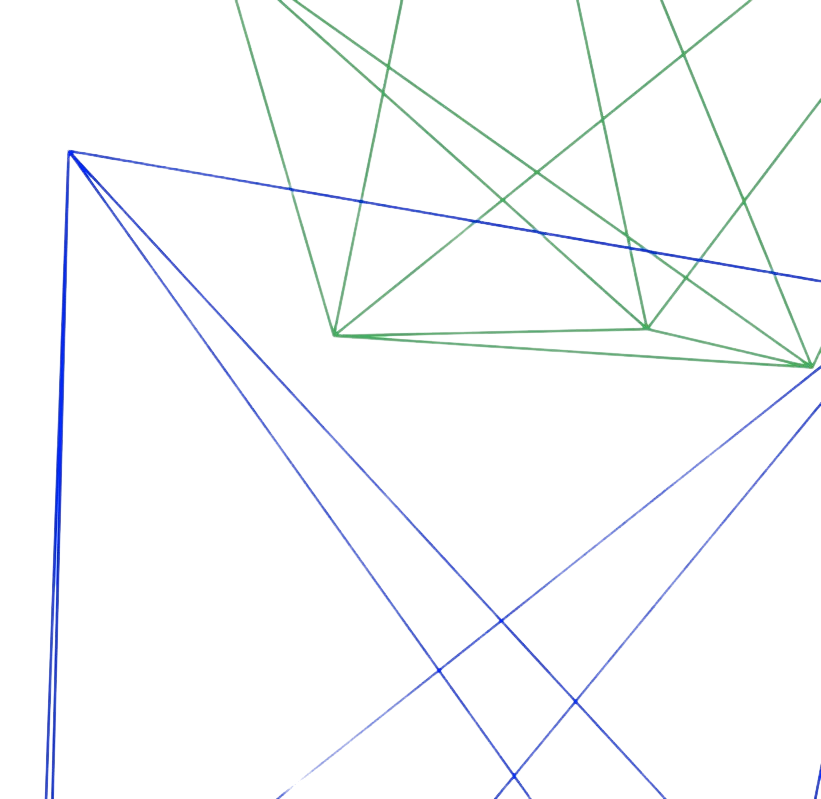
\includegraphics[width=0.5\paperwidth,height=\paperheight]{/root/.config/latex-utils/logos/invert1.png}};

        \node[opacity=0.07,inner sep=0pt, anchor=north west] at (current page.north west){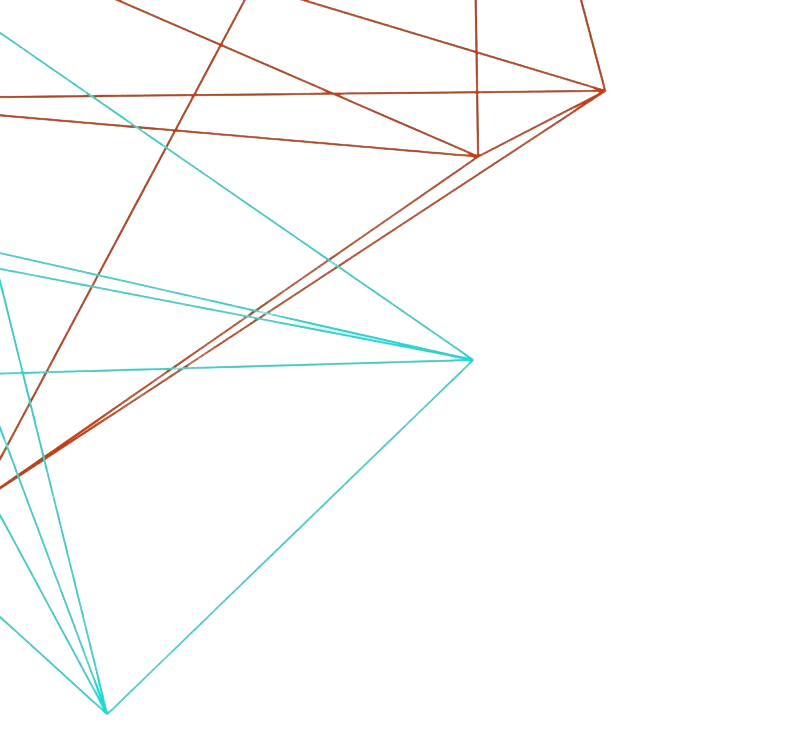
\includegraphics[width=0.5\paperwidth,height=0.5\paperheight]{/root/.config/latex-utils/logos/invert3.png}};




        \node at (page cs:0,0.345) {\Large\textsc{High School Observation and Learning Internship}};
        \node at (page cs:0,0.875) {\Large\bfseries\textsc{Observation Internship}};
        \node at (page cs:0,0.925) {\LARGE\bfseries\textsc{Lycée Français de Barcelone}};

        \node at (page cs:0.5,0) {\Large\textsc{Cyril Lescure - Pedagogical Tutor}};








        %\node[opacity=0.15, inner sep=0pt, anchor=south west] at (current page.south west){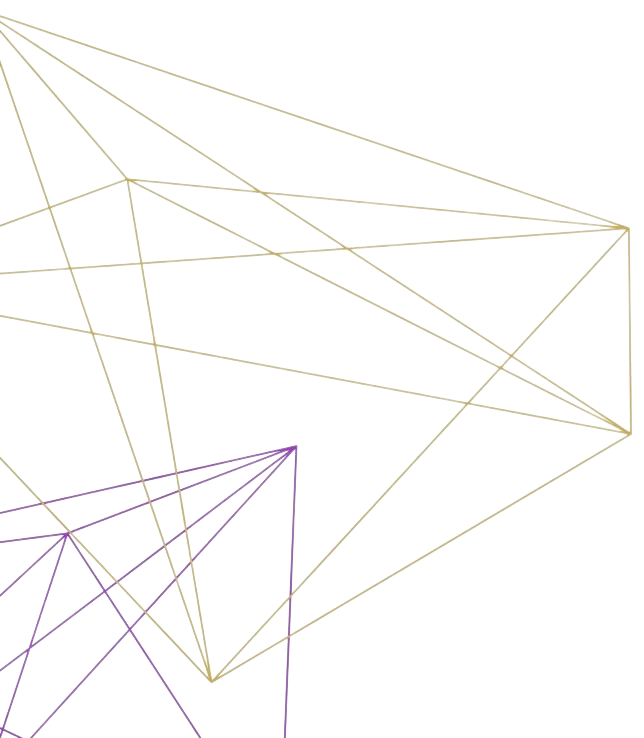
\includegraphics[width=0.5\paperwidth,height=0.5\paperheight]{/root/.config/latex-utils/logos/invert2.png}};

        \node at (page cs:0,0.5) {\fontsize{28}{28.8}\textbf{\ctoptitle}};
        \node at (page cs:0,0.425) {\fontsize{28}{28.8}\textbf{\ctitle}};
        \draw (page cs:0.5,0.375) -- (page cs:-0.5,0.375);
        \node at (page cs:0,0.245) {\LARGE\textsc{\cautor}};
        \node at (page cs:0,0.310) {\Large\textsc{03.06.2019 - 07.06.2019}};


    \end{tikzpicture}
\end{titlepage}


\newgeometry{width=18.625cm, bottom=2cm, top=2cm}

\tikz[remember picture, overlay] \node[opacity=0.3,inner sep=0pt, anchor=north east] at (current page.north east){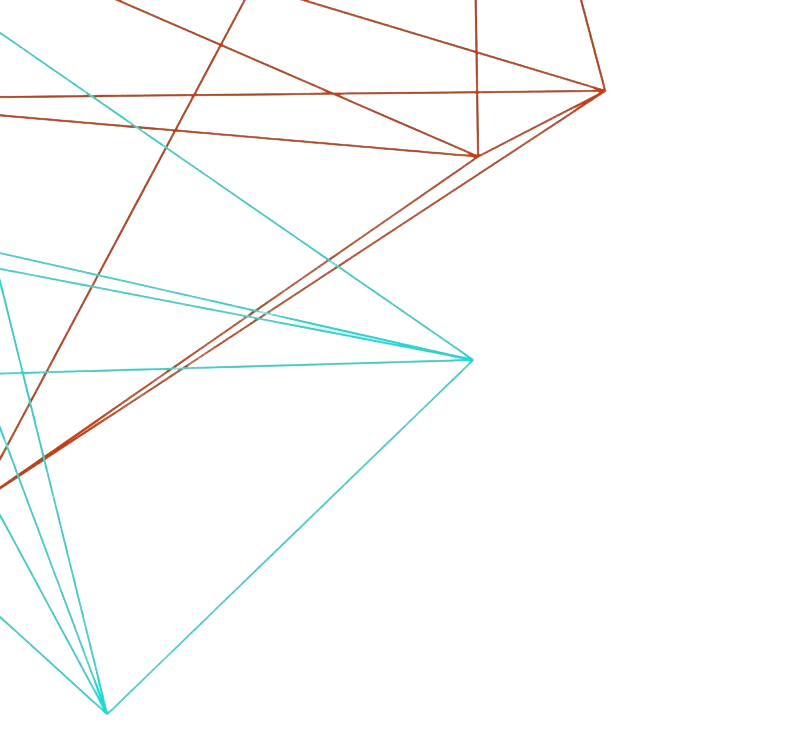
\includegraphics[angle=-90,origin=c,width=0.5\paperheight,height=0.5\paperwidth]{/root/.config/latex-utils/logos/invert3.png}};
\tikz[remember picture,overlay] \node[opacity=0.3,inner sep=0pt, anchor=south east] at (current page.south east){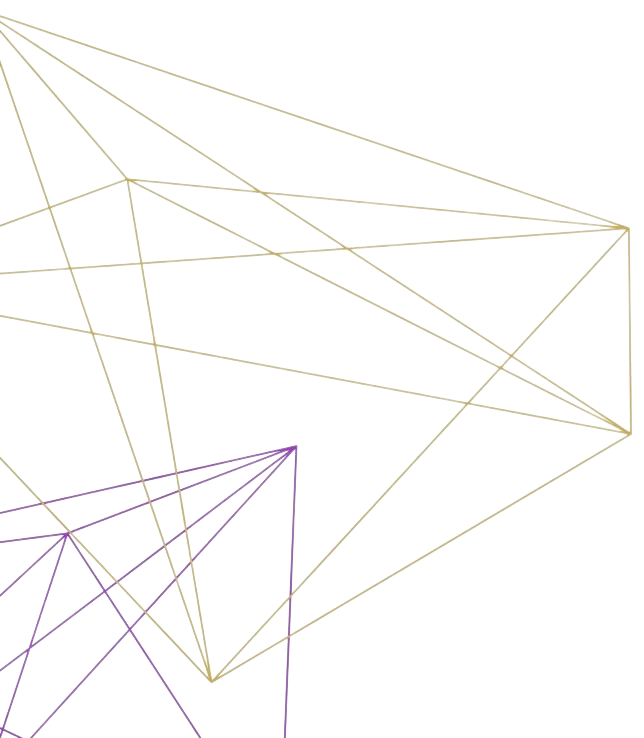
\includegraphics[angle=90,width=0.5\paperwidth,height=0.5\paperheight]{/root/.config/latex-utils/logos/invert2.png}};

\tableofcontents





\vspace*{\fill}
\section{Introduction}

\tab The International Thermonuclear Experimental Reactor (ITER) is an international project aiming to create the world's biggest nuclear fusion reactor. Located in Aix-en-Provence, it's intended to produce over 10 times more output energy than its input. However, this is by no means going to be a commercially used reactor. Due to its experimental nature, its main purpose is to provide a laboratory environment where fusion plasma can be further tested to find the most optimized fusion formula for a commercially used reactor, Demo.

\tab On a first note, we'll be exploring the different types of magnetic confinements, explaining why we chose a tokamak-like build over other possible builds such as the stellarator. Next, we'll take a keen interest in the systems responsible for the safety and diagnostics of the reactor, ensuring that every element of the reactor is controlled and monitored.\\
\tab Later, we'll talk a little about fusion and its reactions, why and which ones we plan to use, as well as find out whether it's safer to operate than our modern-day fission reactors.
And lastly, we'll see how to start up the reactor, later going in-depth with calculation verifying that ECRH beams heating the plasma do so the right way, avoiding melting the tungsten walls.


\newpage

\section{Tokamak Design}

\subsection{Types of reactor}

\tab The main difference between a stellarator and a tokamak is the obvious magnetic chamber, due to the shape of the superconducting coils. In a tokamak, the superconducting coils are fitted both vertically and horizontally to control the "drift" created by the plasma's current. A force pushing upwards at the top of the reactor. In addition to this, the energy needed to power the tokamak increases over time, which means that after a certain period, the input power will exceed the output, from which point the plasma will no longer be beneficial to produce energy.

\tab The stellarator, in contrast, tries to combine the magnetic fields from the horizontal and vertical coils with the help of helical coils, which, unlike the tokamak design, will only need a stable amount of power to sustain. Unfortunately, it does come with a few inconveniences, the plasma held inside the reactor isn't cylindrical as would be seen in a tokamak The plasma is twisted alongside the magnetic chamber, which is quite a demanding engineering feat. The stellarator might seem all in all a good candidate for nuclear fusion but unfortunately, its design is extremely complex. It could, perhaps, one day become a suitable design for a technologically advanced civilization, but for now we simply lack the technology and knowledge necessary for the development of such reactors

\subsection{Control and monitoring}

\tab Once the plasma is heated it rushes upwards towards the ceiling of the reactor which is an effect called "drift". If the plasma ends up touching the ceiling of the reactor, the number of particles colliding into the beryllium wall will be sufficient to create a force powerful enough to lift the 23 000 ton machine for an instant before dropping back down and hitting the ground with a colossal amount of energy.

\tab An example of such an event happened in the UK, at the Joint European Torus (JET), where the impact was so powerful that seismographs nearby detected it as a small earthquake. This bearing in mind that it only weighs about  2,600 tonnes, about one-tenth of ITER's reactor. We call this consequence a "disruption", and it is considered to be the worst thing that can happen to a reactor since it can effectively destroy the reactor.

\tab Physicists and engineers however manage to control this drift and avoid these disruptions with the help of horizontal coils located both at the top and bottom of the reactor which are capable of powering themselves up and creating a repulsive force on the plasma preventing it from climbing any further. The system controlling this processes data at such a sufficiently rapid rate that it is capable of making millisecond adjustments, ensuring the plasma stays stable.

\tab Other systems also prevent other types of dangerous accidents which could take place during the reaction, a tritium leak would be an example. Tritium being an unstable atom, which means that it is radioactive, is dangerous for the environment and its surroundings. Thankfully a clever system monitoring the pressure inside the valves, and the storage transporting the tritium, can close the entries and exits, making sure that these radioactive particles never escape.

\tab To monitor the plasma inside the tokamak reactor we have diagnostics that acquire information from the tokamak and monitor the behavior of the plasma. They achieve this with the help of a laser system called interferometry. It consists in shooting a laser into the reactor and measuring the phase shifts between a beam inside and outside the reactor. Using this method the diagnosticians can determine the density of the plasma. They can also gather information about the temperature emitted by the plasma and the energy released with the aid of spectroscopy, a graph exposing the different levels of the temperature inside the reactor. This helps them evaluate where the plasma is hottest, and the location of possible impurities trapped inside the plasma.

\tab To monitor the plasma in the machine IT experts have massive server rooms and supercomputers which allow them to process information and rapidly treat the data from instruments inside the reactor. The servers then distribute the information to CODAC where it is monitored and controlled by a team of diagnosticians.

\subsection{The nuclear reaction}


\tab We can achieve fusion using a deuterium-tritium reaction (DT), which then produces helium IV (3.5 MeV) and a neutron (14.1-14.7 MeV). We can also use a deuterium-deuterium (DD) reaction to create helium III (3.5 MeV) and a neutron (2.5 MeV) but we prefer the DT reaction because the neutron emitted is much more energetic than the DD reaction, using this to break lithium VI, creating helium IV and tritium. We then try to keep helium IV in the plasma as long as possible to extract as much energy as possible before it finally flies out and leaves the plasma. Unfortunately, fusion has an important downside, tritium is a rare element to find on Earth and is very much needed to supply the nuclear reactor.

\tab Once the fusion is active a lot of highly energetic neutrons are emitted and need to be managed. Having this in mind, physicists plan to extract the neutrons' energy by using a circuit of water surrounding the reactor. When these neutrons collide with the water molecules, they break the molecular structure creating heat, the circuit of water then turns a turbine as a result of the water heating up and creating convection. A magnet attached to the turbine then converts kinetic energy into electricity by alternating the magnetic field inside a coil. Physicists have also thought of pasting a small layer of uranium which could create fission allowing us to collect even more energy, however, this still remains nothing but an interesting idea.

\subsection{Startup and Safety}

\tab Since fusion is a nuclear reaction some people start to worry whether it might explode since fission reactors have this infamous reputation. However fusion and fission are nothing alike, in nuclear fusion we put a lot of effort into maintaining the reaction, and we try to sustain fusion for as long as possible. With fission, we try to limit the number of reactions taking place, preventing it from getting out of control and exploding. The worst scenario that can happen in a tokamak, other than a disruption, would be encountering a problem preventing us from maintaining the reaction, which would simply halt the fusion reaction. In either case. the plasma inside the reactor simply dissolves and nothing explodes. In the case of a disruption, physicists can measure the gravity of the impact and the damage it caused allowing space for solutions.

\tab Before starting up the reactor physicists try to avoid any impurities, particles and atoms which make the fusion inside the plasma less efficient. Such particles are mostly obtained when the beryllium and tungsten on the walls release out-gases after being exposed to high temperatures.

\tab But other particles such as water can also be accumulating in the inactive nuclear reactor. It is predicted that for ITER the amount of water accumulated inside the tokamak can reach up to 1 liter, which is quite alarming knowing that the plasma must have an overall mass of about 1 gram of matter.

\tab To avoid any impurities the machine is subjected to something called "baking", a process which can take from a few days up to a full week heating the reactor to 200ºC or 320ºC. The metals inside the reactor create out-gases which are then extracted from the reactor with pumps making sure that all the impurities have been purged. After baking, the reactor is subjected to a Glow Discharge Cleaning(GDC) process which is a low-energy plasma absorbing any impurities left behind.




\tab To heat up the reactor and create the plasma we can use 3 different methods:
\begin{items}{-15pt}{-15pt}
    \item Neutral Beam Injection (NBI) which consists of injecting highly energetic particles into the reactor which are then ionized after having collided with another particle giving them their energy and heating the reactor.
    \item Ion Cyclotron Resonance Heating (ICRH) sends electromagnetic waves into the reactor similarly to the way a microwave works. It excites the ions in the reactor, reducing the radius of their circular motion, thus increasing the temperature of the plasma.
    \item Electron Cyclotron Resonance Heating (ECRH) sends electromagnetic waves into the reactor the same way the ICRH does, but targets the electrons instead of exciting the ions, creating more heat that way.
\end{items}



\newpage

\section{ECRH Project}

\tab The ECRH can be described as Gaussian beams, beams with a particular growth which we can calculate with the help of a few equations. In this section, we’ll try to verify that it is heating up properly within the tokamak, both for beams of 170GHz, and 104GHz. To simplify things we will only be doing the calculations for the 170GHz beam.

\tab Here's a little schematic of our situation. Our goal is to determine whether the focal length of the beams, at various points, emitted by the ECRH is enough to both heat the plasma and help physicists determine whether the walls are in danger of melting.

\begin{figure}[ht!]
    \begin{tikzpicture}
        \draw[blue!80!cyan!60,-{Latex[length=5mm, width=3mm]}] (0,-4.5) -- (0,1);
        \draw[blue!80!cyan!60,-{Latex[length=5mm, width=3mm]}] (0,7) -- (0,4);
        \draw[blue!80!cyan!60,-{Latex[length=5mm, width=3mm]}] (0,4) -- (0,1);
        \draw[line width=2pt] (0.1,7.1)  -- (-0.1,6.9);
        \draw[line width=2pt] (-0.1,7.1) -- (0.1,6.9);

        \draw[black!75,dashed] (0,1) arc (270:330:7) arc (330:210:7);
        \filldraw[color=black, fill=gray!50, opacity=0.5] (2.8977,7.7645) arc (375:165:3) -- (2.8977,7.77645);
        \draw (0,-3) arc (270:310:10) arc (310:230:10);
        \draw (-0.75,-5.25) -- (0.75,-3.75);
        \draw (-3.25,-5) -- (-2.25,-4);
        \draw (-3,-2.535826) -- (-4.25,-2.535826) -- (-4.25,-8) -- (1,-8) -- (1,-2.945);
        \draw[red] (-2.85,-8) -- (-2.85,-7.25) -- (-3.05,-4.8) -- (-0.55,-5.05) -- (-1.40616,-0.21803) -- ++ (110.88:8.5);
        \draw[red] (-2.65,-8) -- (-2.65,-7.25) -- (-2.45,-4.2) -- (0.55,-3.95) -- (-0.92320,-0.08863) -- ++ (99.117:4.635);
        \draw[red] (-2.75,-8) -- (-2.75,-4.5) -- (0,-4.5) -- ++ (105:10.7) ;

        \draw[green] (-0.72320,-0.024262) -- (-1.60616,-0.26106);
        \draw[green] (-2.02,1.025676) -- (-1.02,1.29896);
        \draw[green] (-3.925,5.5219) -- (-1.325,6.1381);
        \draw[green] (-3,-7.25) -- (-2.5,-7.25);

        \draw[blue!80!cyan!60] (0,-2.5) arc (90:105:2);

        % Nodes

        \node[green] at (-2.5,1) {$\omega_{res}$};
        \node[green] at (-2,-0.3) {$\omega_{0_2}$};
        \node[green] at (-4.2,5.3) {$\omega_{cs}$};
        \node[green] at (-3.5,-7.5) {$\omega_{0_1}$};
        \node[green] at (-3.5,-7.75) {\tiny$(110\ mm)$};
        \node[blue!80!cyan!60] at (-0.3,-2.3) {$20^{\circ}$};
        \node[red] at (-3.35,-6) {$L_1$};
        \node[red] at (-1.5,-5.25) {$L_2$};
        \node[blue!80!cyan!60, rotate=-90] at (0.25,-0.5) {$3200\ mm$};
        \node[blue!80!cyan!60, rotate=-90] at (0.25,2.5) {$2700\ mm$};
        \node[blue!80!cyan!60, rotate=-90] at (0.25,5.5) {$3500\ mm$};

        \node at (-2,7.25) {Central};
        \node at (-2,6.75) {Solenoid};

        \node[rotate=25] at (3,2) {Resonance};
        \node[rotate=25] at (3.25,1.5) {(Plasma)};



        \node at (-3.25,-4) {Mirror I};
        \node at (-3.25,-4.45) {$(m_1)$};
        \node at (0.25,-5.25) {Mirror II};
        \node at (0.25,-4.85) {$(m_2)$};



    \end{tikzpicture}
\end{figure}





\end{document}